%/ ====================================================================== BEGIN FILE =====
%/ **                                   A N O M A L Y                                   **
%/ =======================================================================================
%/ **                                                                                   **
%/ **  Copyright (c) 2019, Stephen W. Soliday                                           **
%/ **                      stephen.soliday@trncmp.org                                   **
%/ **                      http://research.trncmp.org                                   **
%/ **                                                                                   **
%/ **  -------------------------------------------------------------------------------  **
%/ **                                                                                   **
%/ **  This program is free software: you can redistribute it and/or modify it under    **
%/ **  the terms of the GNU General Public License as published by the Free Software    **
%/ **  Foundation, either version 3 of the License, or (at your option)                 **
%/ **  any later version.                                                               **
%/ **                                                                                   **
%/ **  This program is distributed in the hope that it will be useful, but WITHOUT      **
%/ **  ANY WARRANTY; without even the implied warranty of MERCHANTABILITY or FITNESS    **
%/ **  FOR A PARTICULAR PURPOSE. See the GNU General Public License for more details.   **
%/ **                                                                                   **
%/ **  You should have received a copy of the GNU General Public License along with     **
%/ **  this program. If not, see <http://www.gnu.org/licenses/>.                        **
%/ **                                                                                   **
%/ ----- Modification History ------------------------------------------------------------
%/
%/  @file Anomaly.tex
%/   Provides a description of a method for anomaly detection in high dimensionality data.
%/
%/  @author Stephen W. Soliday
%/  @date 2019-Jul-21 (final)
%/  @date 2019-Jun-25 (draft)
%/
%/ =======================================================================================

\documentclass{article}

\usepackage{amsmath}
\usepackage{amsfonts}
\usepackage{amssymb}
\usepackage{graphicx}
\usepackage{wrapfig}
\usepackage{trncmp}
\usepackage{picinpar}
\usepackage{asiwp}
\usepackage{environ}
\usepackage{fancyvrb}

%  =======================================================================================
% Heading arguments are {volume}{year}{pages}{submitted}{published}{author-full-names}

\jmlrheading{Program Whitepaper}{2019}{}{6/25}{-}{Stephen W.~Soliday}{L3T/ADS}

% Short headings should be running head and authors last names

\ShortHeadings{Anomaly Detection}{Soliday}
\firstpageno{1}
%  =======================================================================================


\begin{document}
\title{Auto-encoding Deep Neural Networks for Anomaly Detection}
\author{ \name Stephen W.~Soliday \email stephen.soliday@sg.l3t.com \\
  \addr L3 Harris Technologies \\ Airborne and Space Systems
}
\date{25-June-2019}

\maketitle

\begin{abstract}%

  Analysts have to sift through thousands of images looking for the one image that may be different.
  This approach uses unsupervised learning to discover relevant features in a mass of similar images.
  The system then sorts the images from least likely to most likely to represent the archetype image.
  Two experiments are performed. One with image data, the second with high dimensional non-image data.
  
\end{abstract}

\vspace{12pt}
\textbf{Keywords}: Auto-encoding, Neural network, Unsupervised

%/ =======================================================================================
\section{Introduction\label{sec:intro}}
%/ =======================================================================================

Present Tense

\begin{enumerate}
\item Provide two UC examples
  \begin{enumerate}
  \item Choose an image task using synthetically generated images.
  \item Choose a non-image high dimensional data set from literature.
  \end{enumerate}
\item say how knowledge gained on this task may not translate to the next.
  Rock/snail followed by nickles/dime.
\item show images
  \begin{enumerate}
  \item waves/wake
  \item rocks and snail
  \item cruise ships/destroyer
  \end{enumerate}
\item Mention prior work on image anomaly detection.
  Show how the train a classifier to identify a finite set of classes.
\end{enumerate}

A typical task for image analysts is to sift through thousands of similar images, looking
for that one image that is different. Deep Neural Networks have been very successful at
learning to classify images, when presented with labeled data.

Imagine that you have a thousand small round stones in you driveway.
Among those thousand stones is one snail, and you must find the snail.
Prior to the task you have no knowledge about either stones or snails.

You would pick up and examine each object. Over time you would come to
understand what attributes or features are common to the mass and what is different.

Within the mass some objects would be the most like the average of the mass and some
objects that are very different from the mass.

Little if anything that you learn in this task may be used in the next task. Maybe next time
your task is to find the one dime in ajar of nickles.


%/ ---------------------------------------------------------------------------------------
\subsection{Background\label{sec:back}}
%/ ---------------------------------------------------------------------------------------

Find 3-5 papers on Autoencodeing, GANN's, and Feature clustering. Discuss their usage and success or failure.

\newpage

%/ =======================================================================================
\section{Auto Encoding Decoding Neural Network\label{sec:autoencoder}}
%/ =======================================================================================

\begin{figure}
  \begin{center}
    \includegraphics[width=4in]{figures/AutoGen.eps}
    \caption{Auto-encoding / decodeing neural network}
    \label{fig:threelayer}
  \end{center}
\end{figure}

Figure\ref{fig:threelayer}, shows the schematic for an auto-encoding/decoding neural network.

Describe the architecture.
what does it do?

\section{Method\label{sec:method}}

\subsection{Synthetic training data}
What is this?

\subsubsection{3-D Models}
AC3D and Blender

\begin{figure}
  \begin{center}
    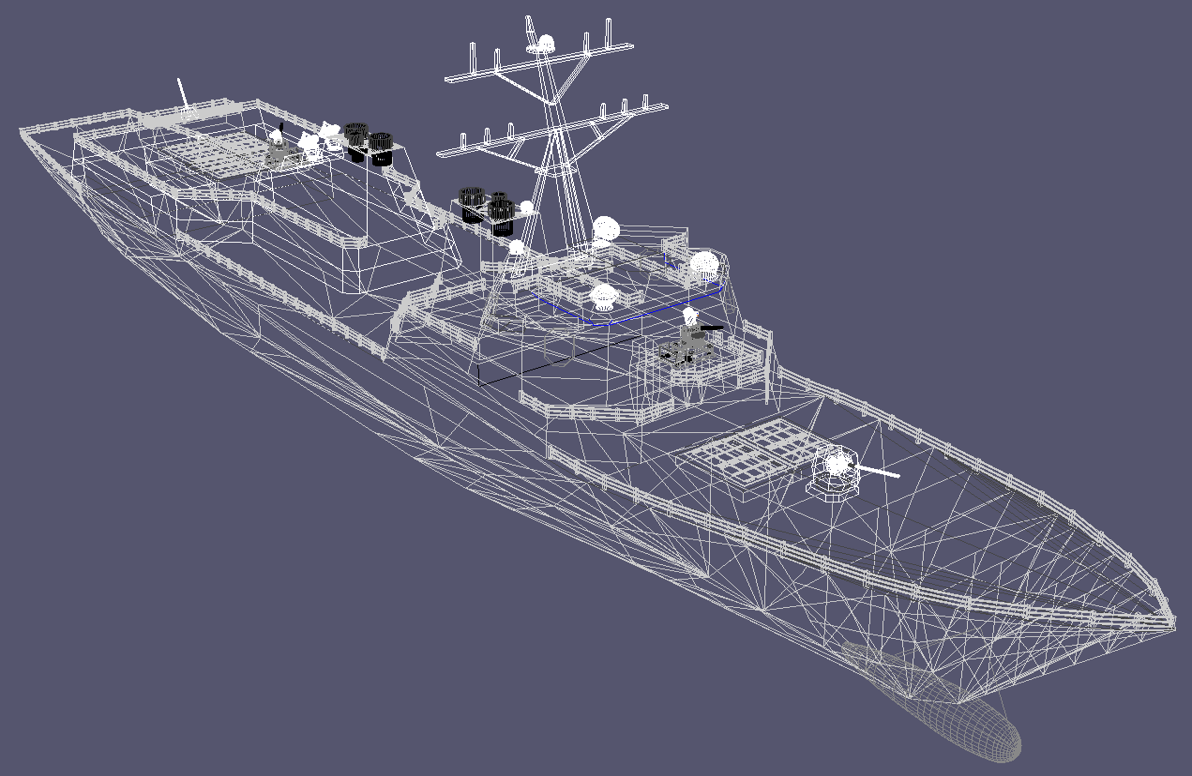
\includegraphics[width=3in]{images/Wireframe.eps}
    \caption{Wireframe Diagram of DDG-51 USS Arleigh Burke}
    \label{fig:threelayer}
  \end{center}
\end{figure}

\subsubsection{Raytracing}
PovRay, python scripts. Discuss: Camera angle, Sun Angle, and Sea State.

\begin{figure}
  \begin{center}
    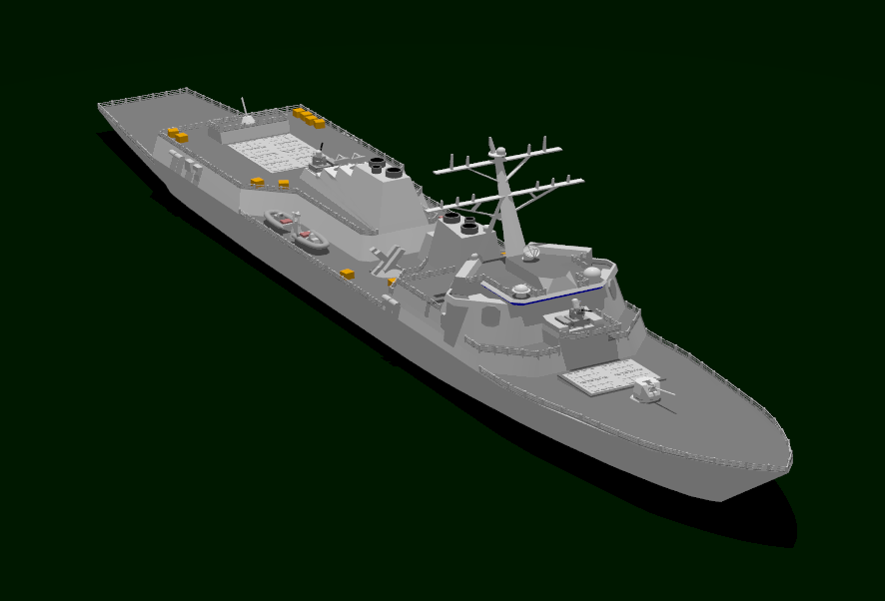
\includegraphics[width=3in]{images/Rendered.eps}
    \caption{PovRay Rendered Image of DDG-51 USS Arleigh Burke}
    \label{fig:threelayer}
  \end{center}
\end{figure}
\begin{figure}
  \begin{center}
    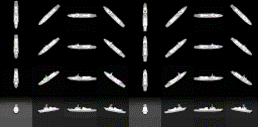
\includegraphics[width=2in]{images/Chips.eps}
    \caption{Selection of chips with various camera and sun angles}
    \label{fig:threelayer}
  \end{center}
\end{figure}

\subsubsection{Training, Validation, Testing}
Discuss Quantity and Quantity.

\subsection{Hyperparameter Selection}

\subsection{Alternate Method -- Single Train vs. All Classes}

As an alternative experiment the same architecture was used with a different work flow.
To review. The work flow described above was as follows:
\begin{enumerate}
\item Select a class and a quantity for the mass (e.g. DDG x 1000)
\item Select a class for the anomaly (e.g. Tanker)
\item Train Auto-encoder/decoder to reconstruct all images.
\item Run all images (\textit{ mass and anomaly }) through encoder only creating a corresponding list of feature vectors.
\item Generate a mean feature vector and a covariance matrix from the feature vectors.
  \item find the Mahalanobis distance of each feature vector from the mean vector and sort in descending order of distance.
\end{enumerate}

As an alternative work flow, the following was tried:
\begin{enumerate}
\item Select an existing unlabeled data set of images similar to targets, non-targets and clutter. In this case one thousand chips of each of the four classes was used.
\item Train Auto-encoder/decoder to reconstruct all images.
\item Select a class and a quantity for the mass (e.g. DDG x 1000)
\item Select a class for the anomaly (e.g. Tanker)
\item Run all images (\textit{ mass and anomaly }) through encoder only creating a corresponding list of feature vectors.
\item Generate a mean feature vector and a covariance matrix from the feature vectors.
  \item find the Mahalanobis distance of each feature vector from the mean vector and sort in descending order of distance.
\end{enumerate}

The disadvantage of this second work flow is that it requires you to posses exemplar data.


\newpage

%/ =======================================================================================
\section{Results\label{sec:results}}
%/ =======================================================================================

past tense

evaluation and commentary on your data.

Introduce a graphic by name
show it
interpret it

Describe each run and choice of hyper parameters

What are the value of each metric


%/ =======================================================================================
\section{Discussion\label{sec:discuss}}
%/ =======================================================================================

Present Tense

How did the results support your introduction
The anomalous image was always in the top 20 out of 1000
how did it improve - that analys need not look at all 1000 images

Do not introduce new ideas here.


%/ =======================================================================================
\subsection{Conclusions and Recommendations\label{sec:conclude}}
%/ =======================================================================================

make some subjective statements

next efforts

\nocite{savitsky:03}





%/ =======================================================================================
\section*{References\label{sec:cites}}
%/ =======================================================================================

\bibliography{soliday}

%/ =======================================================================================
%\section{Appendices\label{sec:apendix}}
%/ =======================================================================================


%  ==========================================================================================

%\newpage
%../common/soliday-bio.tex 

%\begin{verbatim}
%http://www2.fiu.edu/~sabar/enc1102/Research%20Paper%20Advice.htm
%http://tychousa8.umuc.edu/WRTG999A/index.html
%\end{verbatim}

\end{document}

%/ =======================================================================================
%/ **                          H E A D I N G S P E E D . T E X                          **
%  ======================================================================== END FILE =====
